% ============================================================================
% 系统架构与问题建模 - 03_system_architecture.tex
% ============================================================================

\section{问题表述与建模}
\label{sec:system_architecture}

本节把模糊的现实安全问题转化为可量化、可建模的标准化数学问题。通过构建城市低空无人机路径规划的数学框架，将现实世界抽象为可计算的时空张量场，定义无人机的状态演化规律，并将路径规划问题形式化为带约束的多目标优化问题。环境风险因子的详细物理推导将在第4节展开。

\subsection{城市低空四维时空环境定义}

为实现算法的栅格化搜索，首先将连续的三维空间 $\mathcal{V} \subset \mathbb{R}^3$ 和连续时间域 $\mathcal{T} = [0, T_{max}]$ 离散化为四维张量网格：
\begin{equation}
\mathcal{G} = \{ (x, y, z, t_k) \mid x \in X, y \in Y, z \in Z, t_k = k \cdot \Delta t \}
\end{equation}
其中，$\Delta t$ 为时间切片分辨率，$k$ 为时间切片索引。

在任意时空节点上，环境风险被封装为一个多维风险元组：
\begin{equation}
\mathcal{R}_{env}(x, y, z, t) = \big\langle P_{crash}, R_{fatality}, R_{property}, R_{noise} \big\rangle
\end{equation}
这四项因子的详细物理推导将在第4节详述。

\begin{figure}[t]
    \centering
    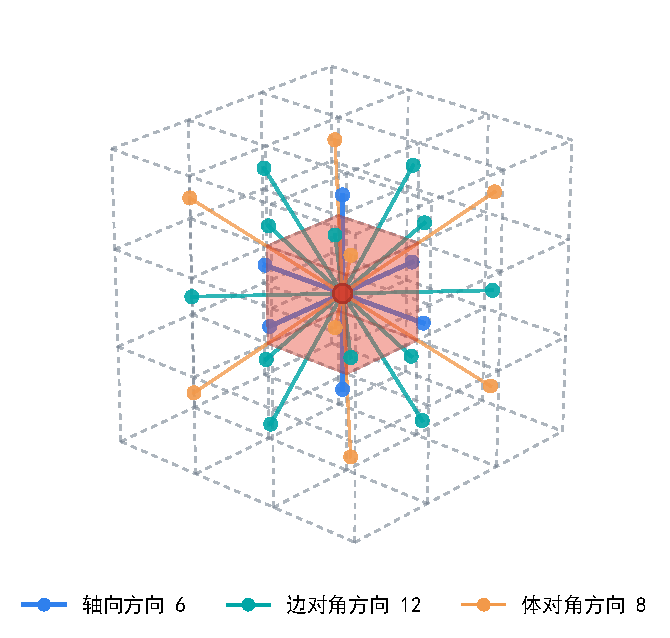
\includegraphics[width=0.48\textwidth]{figures/figure1_26_neighbors.pdf}
    \caption{26-neighbor voxel connectivity.}
\end{figure}

\begin{figure}[htbp]
    \centering
    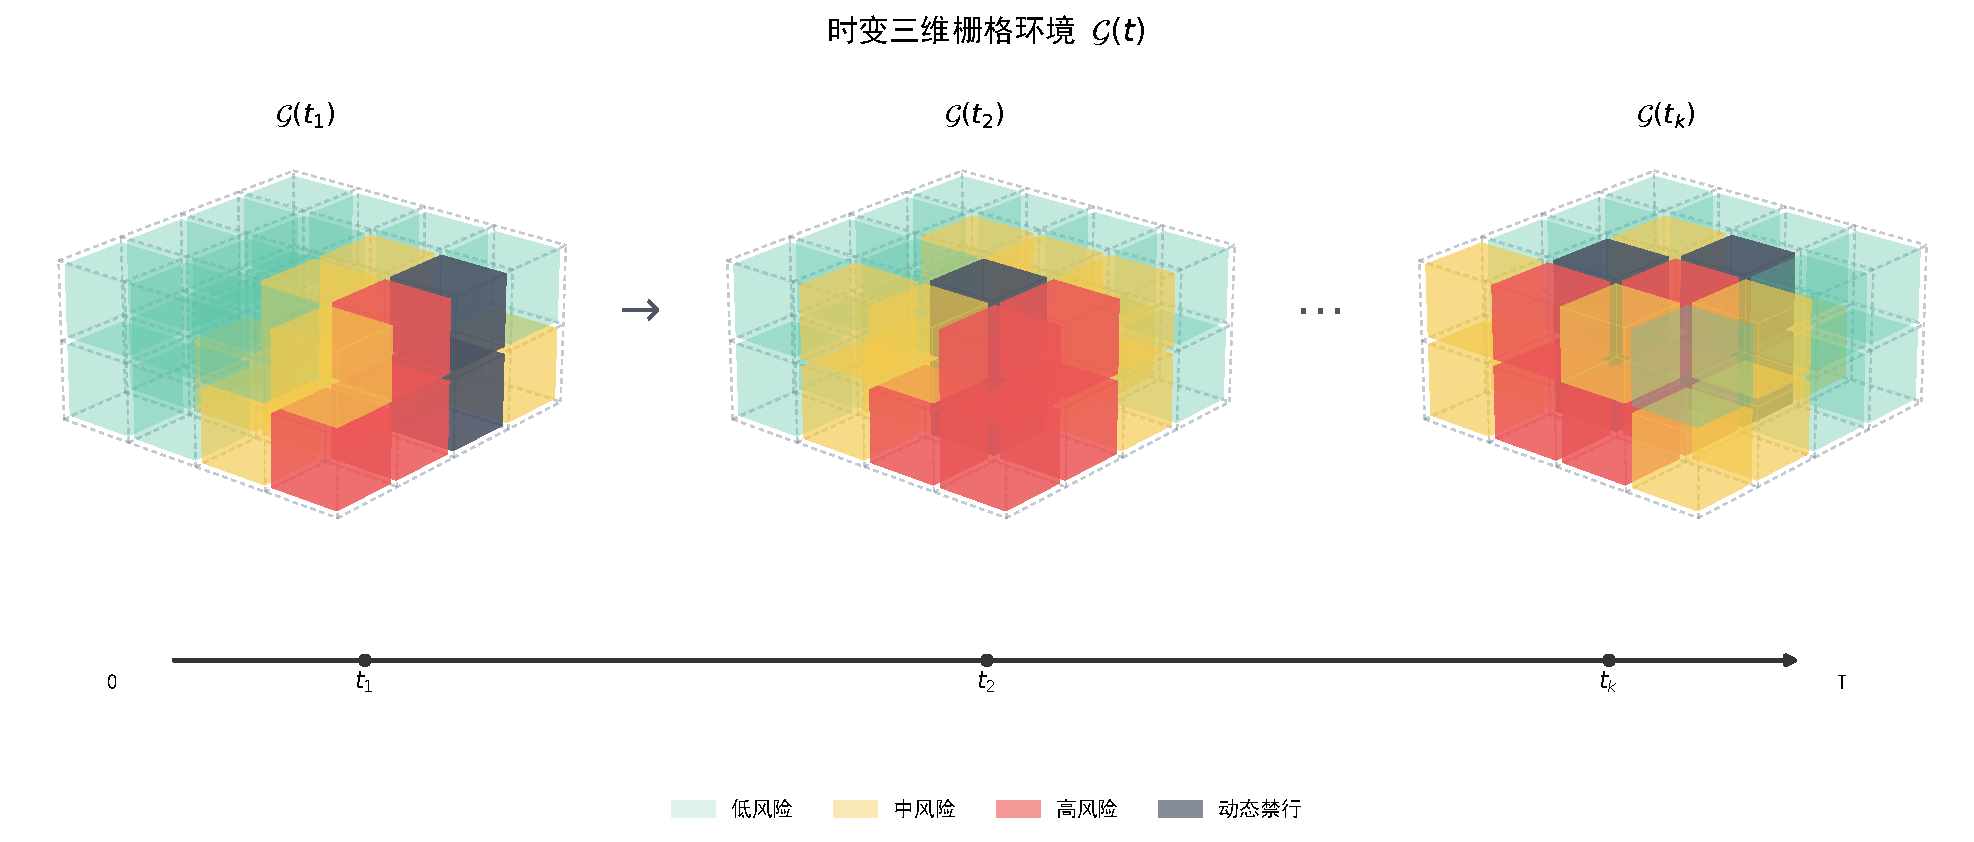
\includegraphics[width=0.8\linewidth]{figures/spacetime_grid_evolution.pdf}
    \caption{时空网格演化}
    \label{fig:spacetime_evolution}
\end{figure}


\subsection{无人机状态向量设计与时空演化}

\subsubsection{状态向量的定义}

定义无人机在路径中第 $i$ 步的完整状态向量 $S_i$：
\begin{equation}
S_i = \left[ \mathbf{p}_i, t_i, \mathbf{\Psi}_i \right]^T
\end{equation}
其中 $\mathbf{p}_i = (x_i, y_i, z_i)$ 为空间坐标；$t_i$ 为到达该点的绝对时间；$\mathbf{\Psi}_i$ 为累积风险状态元组，定义为：
\begin{equation}
\mathbf{\Psi}_i = \left[ P_{surv}^{(i)}, C_{fatality}^{(i)}, C_{property}^{(i)}, C_{noise}^{(i)} \right]
\end{equation}

\subsubsection{时间推演方程}

当无人机由节点 $S_i$ 飞往相邻节点 $S_{i+1}$ 时，时间属性的更新法则为：
\begin{equation}
t_{i+1} = t_i + \Delta t_{fly}^{(i)} = t_i + \frac{\|\mathbf{p}_{i+1} - \mathbf{p}_i\|_2}{v_{uav}}
\end{equation}
其中 $v_{uav}$ 为无人机的巡航速度，$\Delta t_{fly}^{(i)}$ 为第 $i$ 步的飞行耗时，其值取决于相邻节点的空间位移。

\subsubsection{存活概率的马尔可夫演化}

无人机到达第 $i+1$ 步时的累积存活概率，等于它存活到达第 $i$ 步的概率，乘以它在当前航段 $(S_i \rightarrow S_{i+1})$ 上不发生系统失效的概率：
\begin{equation}
P_{surv}^{(i+1)} = P_{surv}^{(i)} \times \big( 1 - P_{crash}(\mathbf{p}_{i+1}, t_{i+1}) \big)
\end{equation}
结合前文提出的动态比例风险模型，该演化过程可严密表达为时间积分的离散形式：
\begin{equation}
P_{surv}^{(i+1)} = P_{surv}^{(i)} \cdot \exp\left( -\lambda_{base} \cdot \Phi(\mathbf{p}_{i+1}, t_{i+1}) \cdot \Delta t_{fly}^{(i)} \right)
\label{eq:surv_evolution}
\end{equation}
其中，$\Delta t_{fly}^{(i)}$ 为由节点 $S_i$ 飞往 $S_{i+1}$ 的耗时。

\subsubsection{累积风险代价的加法演化}

各类风险成本的累积本质上是一个基于条件概率的数学期望求和过程。

致死风险与财产风险仅在满足"无人机存活到达该区域"且"在该区域发生坠毁"两个连续条件时才会兑现。因此，其期望代价增量等于到达概率、局部坠毁概率与绝对坠毁后果三者的乘积：
\begin{align}
C_{fatality}^{(i+1)} &= C_{fatality}^{(i)} + P_{surv}^{(i)} \cdot P_{crash}(\mathbf{p}_{i+1}, t_{i+1}) \cdot E_{fatality}(\mathbf{p}_{i+1}, t_{i+1}) \label{eq:fatality_evolution} \\
C_{property}^{(i+1)} &= C_{property}^{(i)} + P_{surv}^{(i)} \cdot P_{crash}(\mathbf{p}_{i+1}, t_{i+1}) \cdot E_{property}(\mathbf{p}_{i+1})
\end{align}
其中，$E_{fatality}$ 和 $E_{property}$ 分别为在局部发生坠机时造成的绝对预期伤亡人数与财产损失值。注意，$P_{crash}$ 已随驻留时间衰减，此处无需重复乘以 $\Delta t_{fly}$。

与碰撞风险不同，噪声滋扰无需以坠毁为前提，只要无人机存活到达该区域并持续飞行，即产生社会影响。因此，其期望代价受限于无人机的存活到达概率，并与驻留时间成正比：
\begin{equation}
C_{noise}^{(i+1)} = C_{noise}^{(i)} + P_{surv}^{(i)} \cdot R_{noise}(\mathbf{p}_{i+1}, t_{i+1}) \cdot \Delta t_{fly}^{(i)}
\label{eq:noise_evolution}
\end{equation}


\subsection{多维目标函数与动态路径规划问题的数学描述}

\subsubsection{基于张量极值的归一化策略}

在多目标路径规划中，代价指标不仅量纲各异，而且数值跨度极大（致死人数 $0\sim0.03$、财产损失 $0\sim553$、噪声 $0\sim1.4$、距离 $0\sim17.3\,\text{m}$）。若直接加权求和，权重系数将被量纲和数值范围扭曲，失去偏好解释能力。

为实现量纲统一，使各权重系数 $w_k$ 具有明确的偏好含义，本文采用张量极值归一化策略。各项代价的归一化分母 $\Omega_{(\cdot)}$ 在搜索前由四维环境张量的全局极值一次性确定，搜索过程中保持不变。定义无人机由节点 $S_i$ 转移至相邻节点 $S_{i+1}$ 时产生的综合代价增量 $\Delta J^{(i)}$ 为：
\begin{equation}
\Delta J^{(i)} = w_1 \Delta \tilde{C}_{fatality}^{(i)} + w_2 \Delta \tilde{C}_{property}^{(i)} + w_3 \Delta \tilde{C}_{noise}^{(i)} + w_4 \Delta \tilde{C}_{dist}^{(i)}
\end{equation}
其中 $w_1, w_2, w_3, w_4$ 为满足 $\sum_{k=1}^4 w_k = 1$ 的偏好权重系数。各项单步代价均通过其在四维时空张量中的理论最大极值进行归一化，确保每一项的值域严格约束在 $[0,1]$ 区间内。

（1）风险期望的归一化

在搜索初始化阶段，从四维环境张量 $\mathcal{G}$ 中提取全局最大风险极值，作为归一化分母：
\begin{align}
\Omega_{fatality} &= \max_{(x,y,z,t) \in \mathcal{G}} \left[ P_{crash}(x,y,z,t) \cdot E_{fatality}(x,y,z,t) \right] \\
\Omega_{property} &= \max_{(x,y,z,t) \in \mathcal{G}} \left[ P_{crash}(x,y,z,t) \cdot E_{property}(x,y,z) \right] \\
\Omega_{noise} &= \max_{(x,y,z,t) \in \mathcal{G}} \left[ R_{noise}(x,y,z,t) \right] \cdot \Delta t_{step\_max}
\end{align}
其中，$\Delta t_{step\_max} = \frac{\sqrt{3}d_{res}}{v_{uav}}$ 为单步允许的最大驻留时间（对应三维对角线运动）。在算法搜索过程中，单步致死、财产与噪音代价的增量被严密地除以对应极值进行归一化：
\begin{align}
\Delta \tilde{C}_{fatality}^{(i)} &= \frac{P_{surv}^{(i)} \cdot P_{crash}(\mathbf{p}_{i+1}, t_{i+1}) \cdot E_{fatality}(\mathbf{p}_{i+1}, t_{i+1})}{\Omega_{fatality}} \\
\Delta \tilde{C}_{property}^{(i)} &= \frac{P_{surv}^{(i)} \cdot P_{crash}(\mathbf{p}_{i+1}, t_{i+1}) \cdot E_{property}(\mathbf{p}_{i+1})}{\Omega_{property}} \\
\Delta \tilde{C}_{noise}^{(i)} &= \frac{P_{surv}^{(i)} \cdot R_{noise}(\mathbf{p}_{i+1}, t_{i+1}) \cdot \Delta t_{fly}^{(i)}}{\Omega_{noise}}
\end{align}
由于存活概率 $P_{surv}^{(i)} \leq 1$ 且 $\Delta t_{fly}^{(i)} \leq \Delta t_{step\_max}$，上述三项归一化结果必然满足 $\Delta \tilde{C}_{(\cdot)}^{(i)} \in [0,1]$。

（2）距离代价的归一化

在 26-邻域的三维网格中，无人机单步移动的最大位移发生在"三维对角线运动"上。设网格分辨率为 $d_{res}$，则单步最大物理距离为 $L_{step\_max} = \sqrt{3} \cdot d_{res}$。单步距离代价归一化为：
\begin{equation}
\Delta \tilde{C}_{dist}^{(i)} = \frac{\|\mathbf{p}_{i+1} - \mathbf{p}_i\|_2}{\sqrt{3} \cdot d_{res}}
\end{equation}
该映射确保了空间位移被约束在 $[0,1]$ 区间：直线移动时代价约 0.577，平面斜线约 0.816，三维对角线恰好为 1.0。距离代价作为基准成本，确保算法始终具有收敛至终点的动力。

\subsubsection{全局最优化问题定义}

无人机沿可行路径 $\pi$ 飞完全程的总目标函数 $J(\pi)$ 定义为整条链路上所有单步综合代价增量的累加和：
\begin{equation}
J(\pi) = \sum_{i=0}^{N-1} \Delta J^{(i)}
\end{equation}
在满足无人机动力学与绝对安全阈值的前提下，寻找最优时空轨迹 $\pi^*$，使得：
\begin{equation}
\pi^* = \arg \min_{\pi \in \Pi_{valid}} J(\pi)
\end{equation}
其中可行轨迹空间 $\Pi_{valid}$ 需满足以下硬性约束。

\subsubsection{约束条件}

为确保规划出的时空轨迹在拓扑连接上连续有效，且在物理与动力学上切实可行，可行轨迹空间 $\Pi_{valid}$ 中的任意路径 $\pi = \{S_0, S_1, \dots, S_N\}$ 必须严格满足以下两类约束：

\paragraph{（1）拓扑与网络流守恒约束}
该类约束用于确保路径的起点、终点一致性及空间连续性，等效地满足了混合整数线性规划（MILP）框架下的网络流守恒约束：
\begin{align}
& \mathbf{p}_0 = \mathbf{p}_{start}, \quad \mathbf{p}_N = \mathbf{p}_{goal} \label{eq:con_endpoint} \\
& \mathbf{p}_{i+1} \in \mathcal{N}_{26}(\mathbf{p}_i) \quad \forall i \in [0, N-1] \label{eq:con_continuity} \\
& \mathbf{p}_i \neq \mathbf{p}_j \quad \forall i \neq j \label{eq:con_loopfree}
\end{align}
其中，式(\ref{eq:con_endpoint})确保无人机从指定的起点出发并最终精确抵达终点；式(\ref{eq:con_continuity})要求路径序列中的相邻节点必须在空间上满足26-连通邻域（$\mathcal{N}_{26}$）关系，保证物理飞行的连续性；式(\ref{eq:con_loopfree})禁止路径中出现重复节点，确保生成的轨迹无环（Loop-free）。

\paragraph{（2）物理安全与动力学约束}
作为本研究核心的风险感知体现，时空路径必须符合城市低空飞行的物理红线：
\begin{align}
& \mathbf{p}_i \notin \mathcal{U}_{cba} \quad \forall i \in [0, N] \label{eq:con_obstacle} \\
& P_{surv}^{(i)} \ge P_{th} \quad \forall i \in [0, N] \label{eq:con_survival} \\
& \sum_{i=0}^{N-1} \|\mathbf{p}_{i+1} - \mathbf{p}_i\|_2 \le L_{max} \label{eq:con_battery}
\end{align}
式(\ref{eq:con_obstacle})为建筑体硬隔离约束，确保飞行器不穿透任何被城市建筑物占用的静态网格集合 $\mathcal{U}_{cba}$；式(\ref{eq:con_survival})为强制安全熔断约束，$P_{th}$ 为系统能容忍的最低累积存活概率，一旦在极端天气下 $P_{surv}$ 跌破此阈值，路径将被强行否决；式(\ref{eq:con_battery})为电池动力学约束，确保总实际飞行里程不超过无人机的最大续航上限 $L_{max}$。
